\section{What a pixel measures}\label{sec:pixel}

\begin{quote}
\textbf{In plain words.} You cannot feel gravity while falling freely, and
neither can a detector. What can be felt is the \emph{difference} in gravity
between one place and the next: it stretches things along one direction and
squeezes them along another. That stretching is all a gravitational detector
ever measures.
\end{quote}

A freely falling observer feels no gravitational field at their own position.
What remains measurable is how the field differs between nearby points: the
tidal field. For an observer at rest, with proper time $t$ and coordinates
$x^0 = ct$, $x^i$, it is the symmetric tensor
\begin{equation}\label{eq:tidal}
\tE_{ij} = c^2 R_{0i0j},
\end{equation}
where $R$ is the Riemann curvature tensor, with signature $-{+}{+}{+}$ and
$R^\alpha{}_{\beta\gamma\delta} = \partial_\gamma\Gamma^\alpha_{\beta\delta} - \dots$. The
factor $c^2$ gives $\tE_{ij}$ the units $\mathrm{s^{-2}}$. Two free particles separated by a
small vector $\xi^i$ accelerate relative to one another by
\begin{equation}\label{eq:deviation}
\frac{\dd^2 \xi^i}{\dd t^2} = -\tE_{ij}\,\xi^j .
\end{equation}
Figure~\ref{fig:tidal} shows what this does to a ring of free particles, and
Fig.~\ref{fig:tidal-field} the field around masses and in a wave.

\begin{figure}
\centering
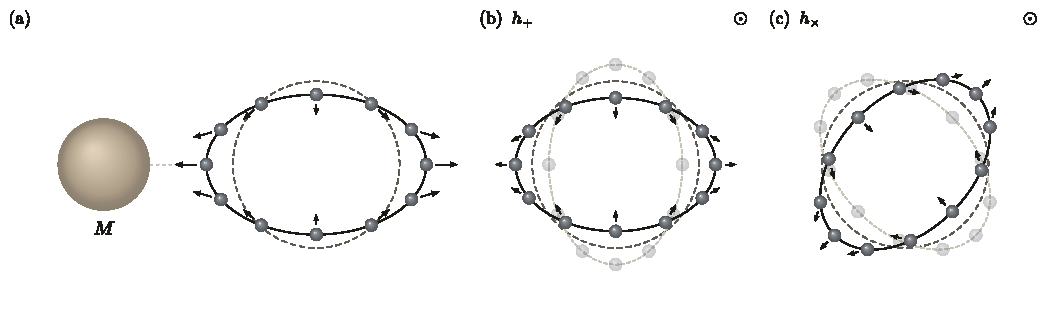
\includegraphics[width=\columnwidth]{figures/tidal.pdf}
\caption{What a pixel measures: a ring of twelve free test masses, distorted by the
tidal field, Eq.~\eqref{eq:deviation}, with each arrow the displacement of
its mass and the dashed circle the ring undisturbed; the distortions are
exaggerated. (a) Beside a mass $M$, the ring is stretched along the line to the
mass and squeezed across it, exactly twice as strongly along as across.
(b), (c) In a gravitational wave travelling toward the reader ($\odot$), of
polarization $h_+$ and $h_\times$: the ring is stretched and squeezed equally
along two perpendicular directions, which change places every half cycle (the
pale ring), and the two polarizations differ by a turn of $45^\circ$. The
planet's size and distance are schematic. A pixel records the size and
orientation of this distortion.}\label{fig:tidal}
\end{figure}

\begin{figure*}
\centering
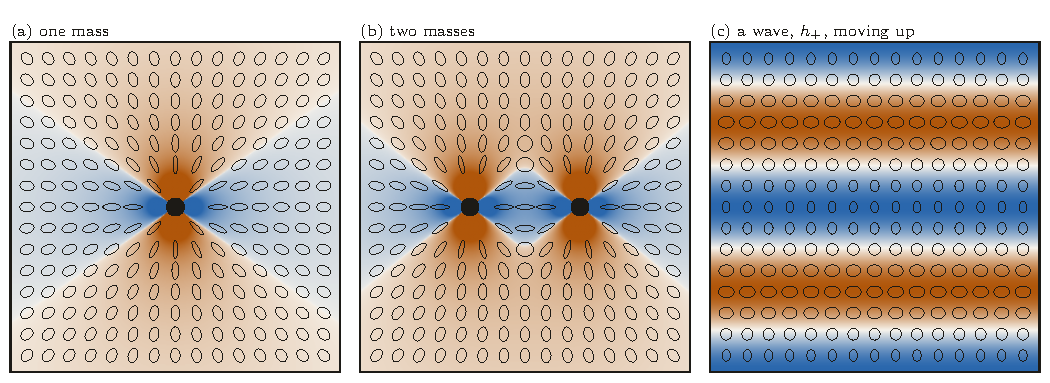
\includegraphics[width=\textwidth]{figures/tidal-field.pdf}
\caption{The tidal field itself. At points of a plane, a small ring of free
particles is drawn as the field distorts it (exaggerated, with the strength
compressed so that weak regions remain visible), over a map of one component:
$\tE_{zz}$ (up the page) in (a) and (b), $\tE_{xx}$ (across) in (c). Orange
marks a stretch along that axis (the component negative, by
Eq.~\eqref{eq:deviation}), blue a squeeze (positive). (a) One mass: every ring is
stretched toward it. (b) Two masses: midway between them the ring is stretched
along the line joining them and squeezed across it. (c) A plane wave of
polarization $h_+$ travelling up the page: bands of stretch and squeeze across
the direction of travel alternate every half wavelength, and nothing happens
along it. A pixel records one such ring, in three dimensions.}\label{fig:tidal-field}
\end{figure*}

Two limits of Eq.~\eqref{eq:tidal} matter here. Close to slowly moving matter,
the tidal field is the second derivative of the Newtonian potential $\Phi$:
\begin{equation}\label{eq:newton}
\tE_{ij} = \partial_i \partial_j \Phi .
\end{equation}
For a body of mass $M$ at distance $r$ its size is $2GM/r^3$ along the line to
the body. Far from its source, in a gravitational wave of strain
$h_{ij}^{\TT}$ (in the transverse traceless gauge),
\begin{equation}\label{eq:wave}
\tE_{ij} = -\tfrac{1}{2}\,\partial_t^2 h_{ij}^{\TT} .
\end{equation}
An interferometer such as LIGO reads one component of $\tE_{ij}$, integrated
twice in time, as the fractional change $h$ in the length of its arms.

Such a detector therefore responds to the ordinary pull of a passing lorry and
to a wave from a distant collision, and nothing in its one reading tells them
apart. The pull is not small. A person of $70\,\mathrm{kg}$ standing one metre
away produces $\tE \approx 9\times10^{-9}\,\mathrm{s^{-2}}$. If they sway by
five centimetres once a second, the field changes by $3\,\delta r/r$ of
itself, about $1.4\times10^{-9}\,\mathrm{s^{-2}}$, which a detector reads as a
strain $h = 2\,\delta\tE/\omega^2 \approx 7\times10^{-11}$, where
$\omega = 2\pi f$ is the angular frequency, here $2\pi\,\mathrm{s^{-1}}$. The
waves LIGO detects have strains near $10^{-21}$. This is why people and
vehicles must be kept away from its mirrors \cite{ThorneWinstein1999}. The
signal that the observatory removes as contamination is the one that a
near-field camera records.

An ideal pixel records all of $\tE_{ij}$, and also its magnetic counterpart
\begin{equation}\label{eq:magnetic}
\tB_{ij} = \tfrac{1}{2}\,c^2\,\epsilon_{ipq}\,R_{pqj0},
\end{equation}
with $\epsilon_{123} = +1$, which describes how the field twists the axes of
nearby gyroscopes relative to one another \cite{Nichols2011}. In vacuum both
are symmetric and trace-free, so
a pixel yields ten numbers at each instant; with this normalization the two are
equal in size in a plane wave, and $\tB_{ij}$ is $\tE_{ij}$ turned by
$45^\circ$ about the direction of travel. Inside matter the Ricci part of the
curvature adds local information that a pixel in vacuum does not see: the
trace $\mathrm{tr}\,\tE = c^2R_{00} = 4\pi G\rho$ in the Newtonian limit, and an
antisymmetric part of the magnetic tensor, $\tB_{[ij]} = -(4\pi
G/c)\,\epsilon_{ijk}\,\rho v_k$ for matter of density $\rho$ flowing at
velocity $\mathbf v$, which points along the flow. The pixel is also assumed
not to rotate: a frame turning at angular velocity $\Omega$ feels a
centrifugal pseudo-tide of order $\Omega^2$, and the Earth's own turning gives
$5\times10^{-9}\,\mathrm{s^{-2}}$, some thirty thousand times the tide of the
Moon, so gyroscopes must hold the frame still. We call an array of such pixels a
gravitational camera.

\paragraph{What the premise asks.} A pixel of this kind is an old idea. The
gravitational compass, a cluster of free masses read against one another, was
proposed to measure the curvature piece by piece
\cite{Pirani1956,Szekeres1965}; a sphere with several transducers reads the five
numbers of $\tE$ at one place \cite{Forward1971,WagonerPaik1977}; and a detector
that reads all of $\tE$ has been designed \cite{Paik2016}. In the near field
the premise asks little more than exists. Tides are measured in eotvos,
$1\,\mathrm{E} = 10^{-9}\,\mathrm{s^{-2}}$, and the person a metre away is nine
of them. An atom gradiometer carried over a buried tunnel reaches
$20\,\mathrm{E}$ in ten minutes \cite{Stray2022}; a superconducting one in the
laboratory, $0.02\,\mathrm{E}$ in a second \cite{MoodyPaikCanavan2002}, a
signal-to-noise ratio of five hundred on that person; and a satellite has
carried one as sensitive around the Earth \cite{RummelYiStummer2011}. Two free
masses of a gram, a centimetre apart and read for a second at the standard
quantum limit, would resolve $6\times10^{-14}\,\mathrm{s^{-2}}$, a hundred
thousand times less than the person's tide. The magnetic part asks more. It
can be read by gyroscopes \cite{Nichols2011}, by a gradiometer in motion
\cite{BraginskyCavesThorne1977,MashhoonPaikWill1989} or by light sent both ways
around a loop \cite{Frauendiener2020}, and in a wave it already enters the
response of an interferometer, at first order in the length of its arms over
the wavelength \cite{BaskaranGrishchuk2004}; but near slow matter it is smaller
than the electric part by $v/c$. The waves of moving bodies and the thermal
glow ask far more again, and the glow asks for something that no matter can
supply (Section~\ref{sec:first-image}).

\paragraph{The Earth's own tide.} On the ground the largest tide is the
planet's own, $2GM/R^3 = 3.1\times10^{-6}\,\mathrm{s^{-2}}$ along the vertical,
three hundred times that of the person a metre away. It is steady and known,
and it is subtracted, as the empty room is in Section~\ref{sec:near-field}: the
rooms of this paper are what remains, or rooms in free fall far from any
planet. The planet's turning is in the reading too. A pixel at rest on the
equator moves with the ground at $\Omega R = 465\,\mathrm{m\,s^{-1}}$, over a
planet that turns beneath it, and the two together
(Eq.~\eqref{eq:magnetic-point} and the spin dipole of
Section~\ref{sec:near-field}) give it a magnetic part
$(3GM\Omega/cR^2)(1 - I/MR^2) = 4.8\times10^{-12}\,\mathrm{s^{-2}}$, with $I$
the planet's moment of inertia: seventy thousand times the magnetic part of a
person walking past a metre away at $1.4\,\mathrm{m\,s^{-1}}$. This too is steady, and it is a measurement:
one pixel on the ground reads $I/MR^2$, the number that tells a planet with a
core from one without (Section~\ref{sec:near-field}).

The two parts are best written as one complex matrix, $\mathcal W = \tE +
i\tB$, and Section~\ref{sec:one-pixel} shows how much a single pixel can read
from it. The sections in between follow an array of pixels through the regimes
in which a camera forms images.
